%-------------------------------------------
\begin{frame}%{Literate programming}

\huge{Literate programming}

\end{frame}

%------------------------------------------------------------
\subsection{Introduction}

%-------------------------------------------
\begin{frame}{Introduction}

What is literate programming ?

    Let us change our traditional attitude to the construction of programs: Instead of imagining that our main task is to instruct a computer what to do, let us concentrate rather on explaining to humans what we want the computer to do.

    — Donald E. Knuth, Literate Programming, 1984
\end{frame}

%-------------------------------------------
\begin{frame}{Introduction}

What is literate programming ?

\begin{definition}
"Literate programming is a \textbf{programming paradigm} introduced by Donald Knuth in which a computer program is given an explanation of its logic in a \textbf{natural language}, such as English, \textbf{interspersed with snippets of macros and traditional source code}, from which compilable source code can be generated." Donald Knuth, 1984.
\end{definition}

Wikipedia, 18/08/2020 \url{https://en.wikipedia.org/wiki/Literate\_programming\#Workflow}
\end{frame}


%-------------------------------------------
\begin{frame}{Introduction}

What does it look like ?

\centering\includegraphics[width=10cm]{07_notebook/images/literate_programming.png}

\end{frame}

%-------------------------------------------
\begin{frame}{Introduction}
\begin{columns}

\column{0.5\textwidth}
\centering\includegraphics[width=6cm]{07_notebook/images/literate_programming.png}

\column{0.5\textwidth}
Interactive programming interface allowing to combine both natural and computer languages.
\newline
\newline
In one file:
\begin{itemize}
  \item Explanations
  \item Code
  \item Results
  \item Graphs and plots
\end{itemize}

\end{columns}
\end{frame}

%-------------------------------------------
\begin{frame}{Introduction}

Why using literate programming frameworks ?\newline
\newline
Use cases:
\begin{itemize}
  \item Day to day analyses
  \item Analysis reports
  \item Writing scientific articles
\end{itemize}

\end{frame}

%-------------------------------------------
\begin{frame}{Example of an article entirely written using a notebook}
\begin{columns}

\column{0.3\textwidth}
File (on a repository)\newline
\newline
\centering\includegraphics[width=3cm]{07_notebook/images/article_github.png}

\column{0.3\textwidth}
Published article\newline
\newline
\centering\includegraphics[width=3cm]{07_notebook/images/article_frontiers.png}
%http://dx.doi.org/10.3389/fphys.2018.00787

\column{0.3\textwidth}
Executable file\newline
\newline
\centering\includegraphics[width=3cm]{07_notebook/images/article_nbviewer.png}
%%https://nbviewer.jupyter.org/gist/pauleve/a86717b0ae8750440dd589f778db428f/Usecase%20-%20Mutations%20enabling%20tumour%20invasion.ipynb

\end{columns}
%\centering https://colomoto.github.io/colomoto-docker/

\end{frame}

%-------------------------------------------
%\begin{frame}{Literate programming}
%
%Available frameworks:
%\begin{itemize}
%  \item Rmarkdown / RStudio
%  \item Jupyter (ex-iPython Notebook)
%\end{itemize}
%\newline
%\newline
%Available for many languages (R, Python...)
%\end{frame}

%-------------------------------------------
\begin{frame}{Literate programming}

This session :
\begin{itemize}
  \item Markdown
  \item Rmarkdown / RStudio
  \item Jupyter
\end{itemize}

\end{frame}

%------------------------------------------------------------
\subsection{Markdown}

%-------------------------------------------
\begin{frame}{Markup and markdown}

\begin{definition}
A markup language uses tags to define elements within a document.
\end{definition}
%\newline
%\newline
\vfill
Three different types and usage :
\begin{itemize}
  \item Presentational (used by traditional word-processing systems)
  \begin{itemize}
      \item Markup is invisible
  \end{itemize}
  \item Procedural, provides instructions to process the text (e.g.\ TeX, PostScript)
  \begin{itemize}
      \item Markup is visible and can be directly manipulated by the author.
  \end{itemize}
  \item Descriptive, to label documents parts (e.g.\ LaTeX, HTML, XML...)
  \begin{itemize}
      \item Emphasizes the document structure.
  \end{itemize}
\end{itemize}

\end{frame}

%-------------------------------------------
\begin{frame}{Markdown language}

Markdown is a Lightweight markup language.

Designed to be :
\begin{itemize}
    \item easy to \textbf{write} using any generic text editor (plain-text-formatting syntax)
    \item easy to \textbf{read} in its raw form
\end{itemize}

\end{frame}

%-------------------------------------------
\begin{frame}{Markdown language}

You've probably see it already on GitHub (README), Wikipedia... 

\centering\includegraphics[width=8cm]{07_notebook/images/markdown.png}

Github guide : url{https://guides.github.com/features/mastering-markdown/}
\end{frame}


%-------------------------------------------
%\begin{frame}{Markdown language}
%
%Une page de wiki est disponible sur FAIR\_bioinfo
%
%https://github.com/thomasdenecker/FAIR\_Bioinfo/wiki/Markdown
%
%\centering\includegraphics[width=8cm]{07_notebook/images/markdown_github_FAIR_bioinfo.png}
%
%\end{frame}

%-------------------------------------------
\begin{frame}{Literate programming}

But how is this useful for literate programming? \newline

When you want to weave both code (to be interpreted) and formatting information, you precisely need a lightweight language for the formatting part.
\end{frame}

%-------------------------------------------
\begin{frame}{The challengers}

No need to hide, there are currently two main frameworks used in bioinformatics:

RMarkdown and Jupyter
\end{frame}

%-------------------------------------------
\begin{frame}{RMarkdown}

\huge{RMarkdown} 

\end{frame}

%-------------------------------------------
\begin{frame}{RMarkdown}
At the beginning, there was nothing. \newline \pause

Then came Sweave.\newline
Leisch, Friedrich (2002). "Sweave, Part I: Mixing R and LaTeX: A short introduction to the Sweave file format and corresponding R functions" \pause

And people saw that the path would be long...
\end{frame}

%-------------------------------------------
\begin{frame}{RMarkdown}
knitR (2011)

\begin{center}
    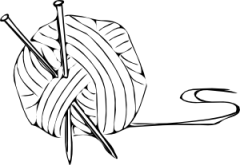
\includegraphics[width=2cm]{07_notebook/images/knitr_logo.png}
\end{center}

"The knitr package was designed to be a transparent engine for dynamic report generation with R, solve some long-standing problems in Sweave, and combine features in other add-on packages into one package"

\url{https://yihui.org/knitr/}

\end{frame}

%-------------------------------------------
\begin{frame}{RMarkdown}
RMarkdown 

\begin{center}
    
\includegraphics[width=10cm]{07_notebook/images/rmarkdown_workflow.png}
\end{center}

"When you run render, R Markdown feeds the .Rmd file to knitr, which executes all of the code chunks and creates a new markdown (.md) document which includes the code and its output. \newline
The markdown file generated by knitr is then processed by pandoc which is responsible for creating the finished format."

\url{https://rmarkdown.rstudio.com}
\end{frame}

%-------------------------------------------
\begin{frame}{RMarkdown}
RMarkdown

\begin{center}
    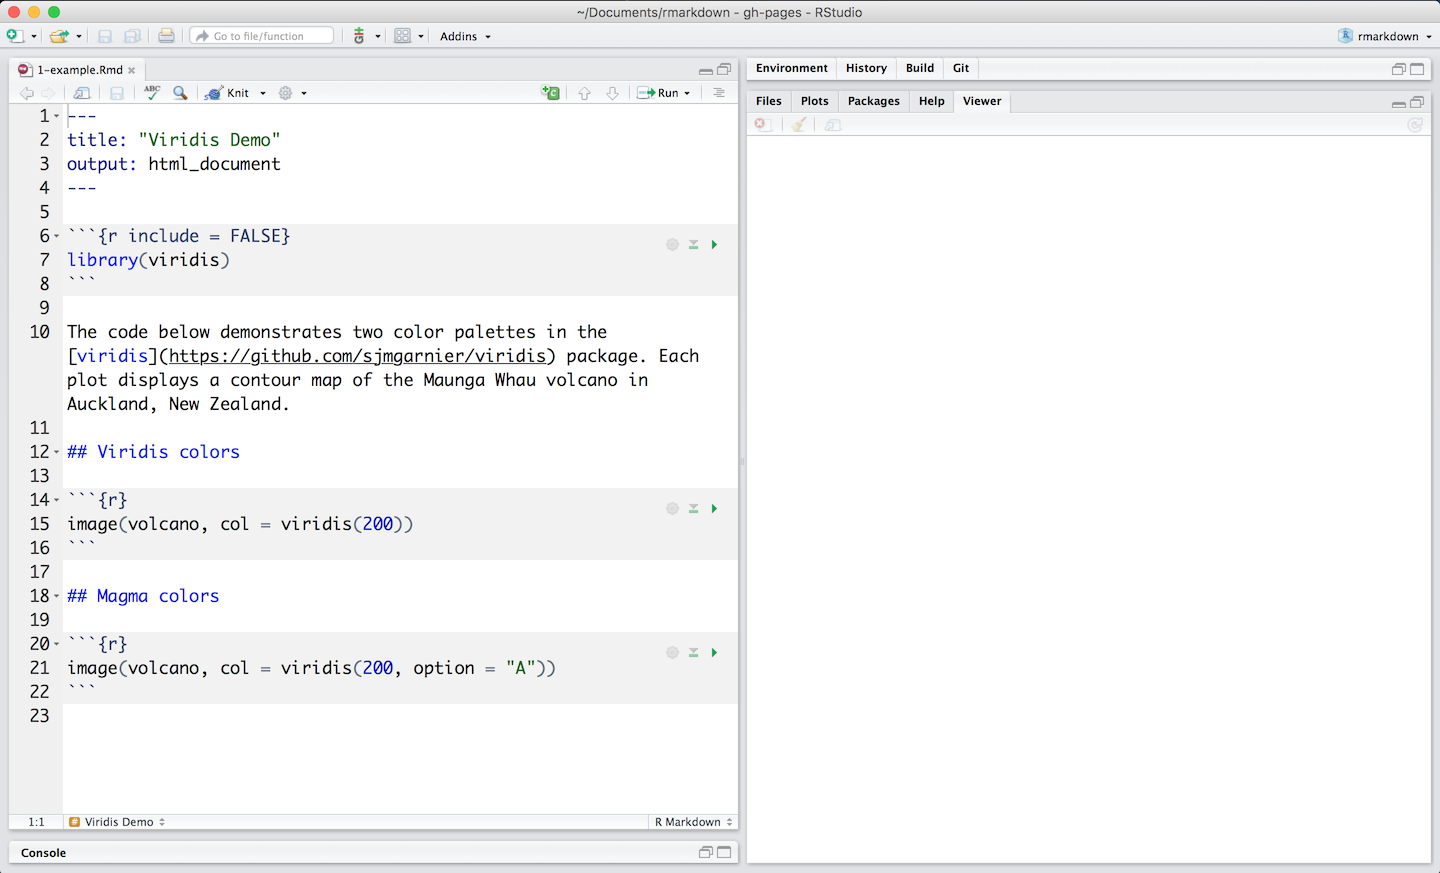
\includegraphics[width=10cm]{07_notebook/images/rmarkdown_file.png}
\end{center}

Integrated into RStudio, IDE for R.

\end{frame}

%-------------------------------------------
\begin{frame}{RMarkdown}
R Notebooks

\begin{center}
    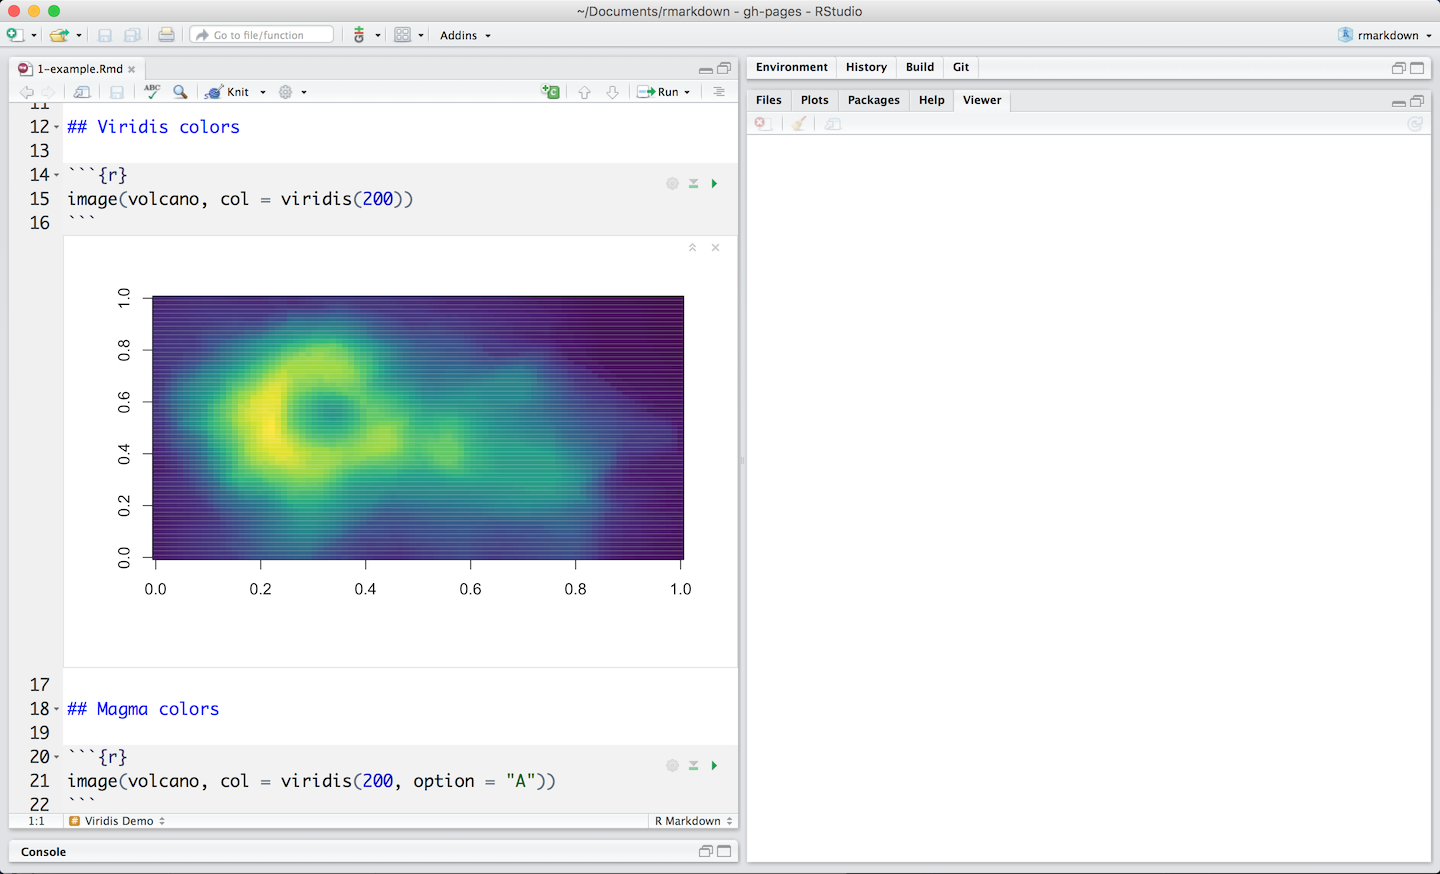
\includegraphics[width=10cm]{07_notebook/images/rmarkdown_notebook.png}
\end{center}


\end{frame}

%-------------------------------------------
\begin{frame}{RMarkdown}
R Notebooks and more...

\begin{center}
    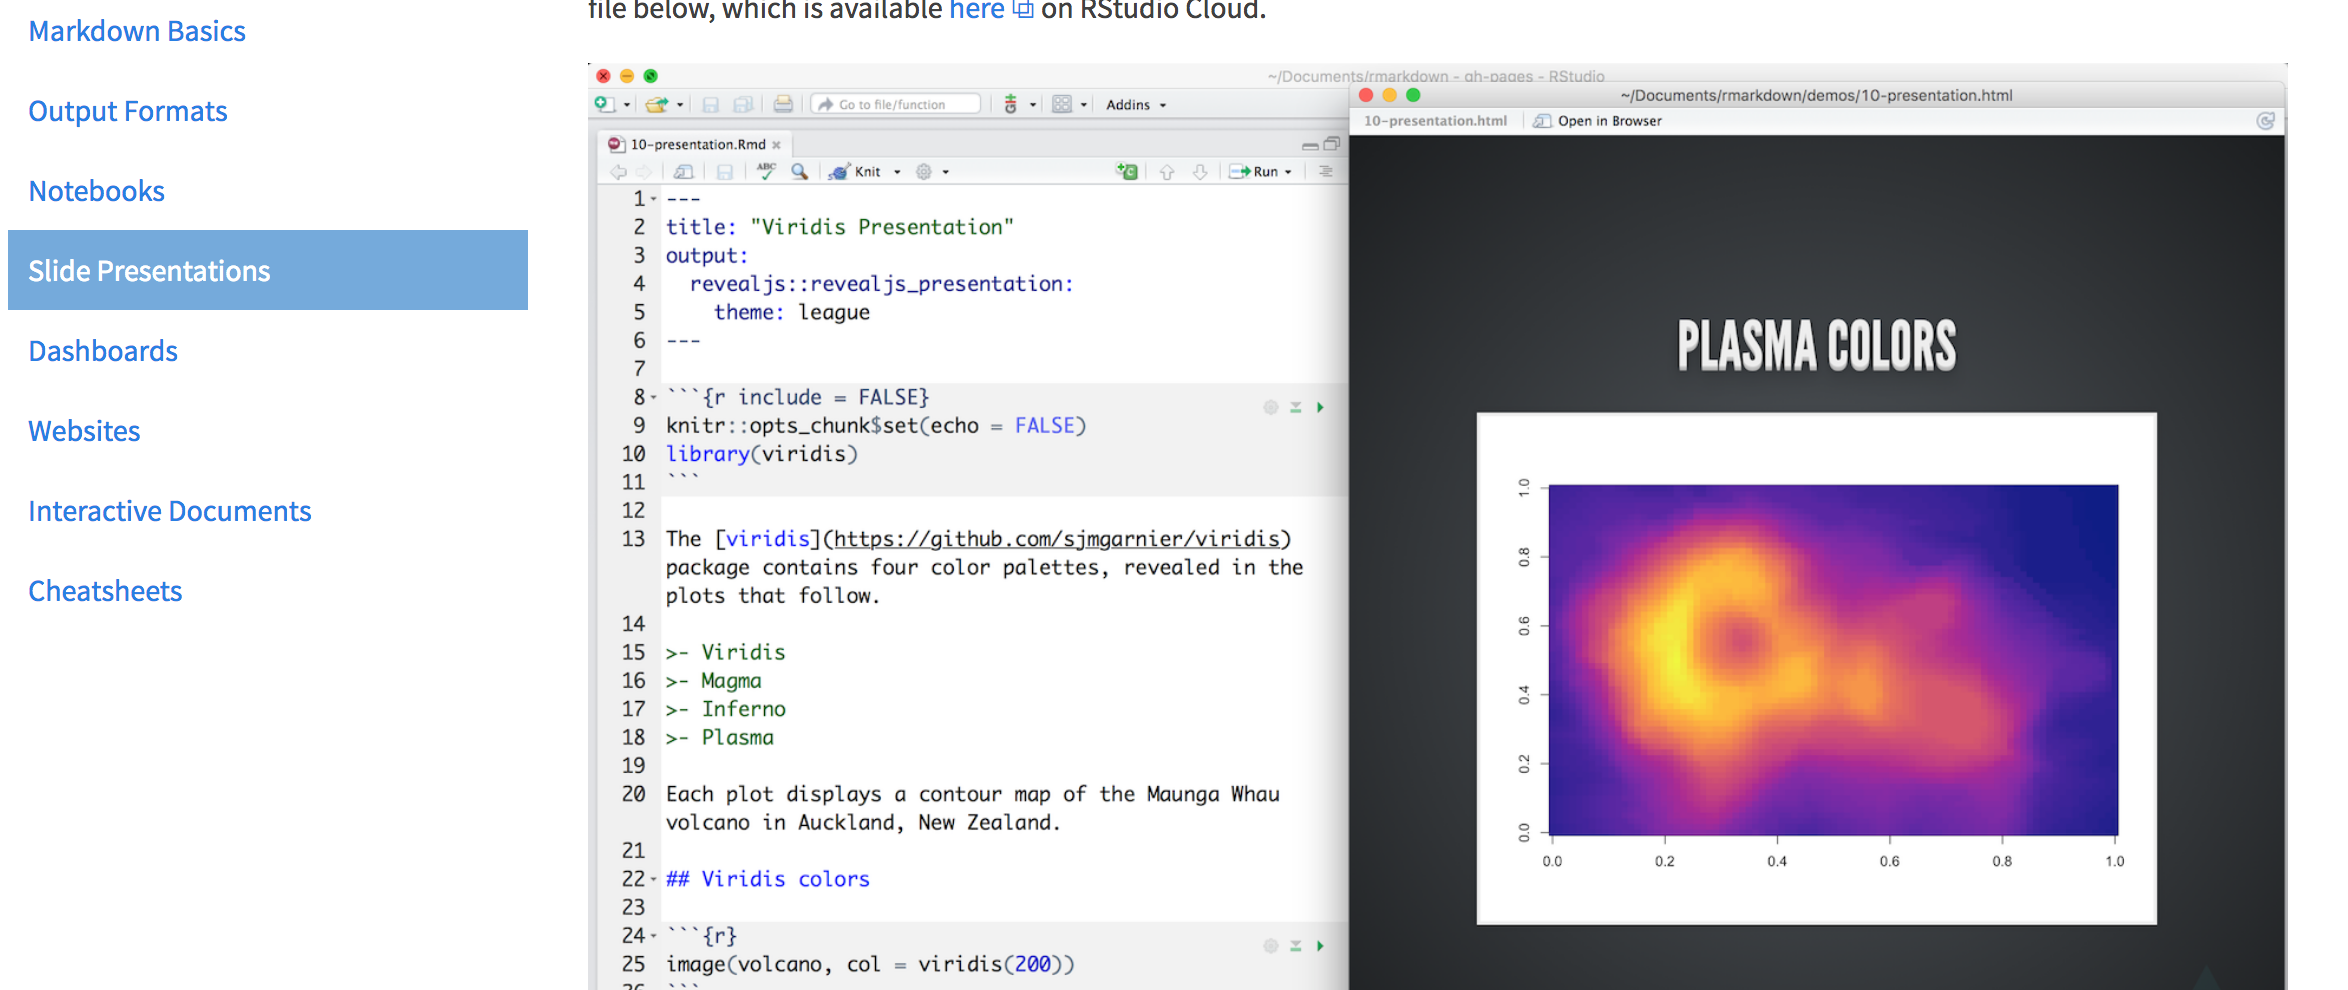
\includegraphics[width=10cm]{07_notebook/images/rmarkdown_etc.png}
\end{center}

\end{frame}

%-------------------------------------------
\begin{frame}{Jupyter}

\huge{Jupyter}

\end{frame}

%-------------------------------------------
\begin{frame}{Jupyter}
A bit of history...
\begin{itemize}
    \item 2011 : IPython (interactive Python shell) with notebook functionalities
    \item 2014 : Spin-off project called Project Jupyter
    \item a non-profit, open-source project maintained by a strong Community
    \item "Jupyter will always be 100\% open-source software, free for all to use and released under the liberal terms of the modified BSD license"
    \item A reference to the three core programming languages supported by Jupyter (Julia, Python and R)
\end{itemize}

\url{https://jupyter.org/}

\end{frame}

%-------------------------------------------
\begin{frame}{Jupyter}
What can it do? \newline \pause
Everything (excepted coffee)
\end{frame}

%-------------------------------------------
\begin{frame}{Jupyter}
But what is it exactly ? \newline \pause
Web-based interactive computational environment. \newline \pause
\begin{itemize}
    \item<3-> Web-based : client/server
    \item<4-> Interactive : notebook system
    \item<5-> Computational environment : console, many kernels available...
\end{itemize}
\end{frame}

%-------------------------------------------
\begin{frame}{Jupyter}
Dashboard

\begin{center}
    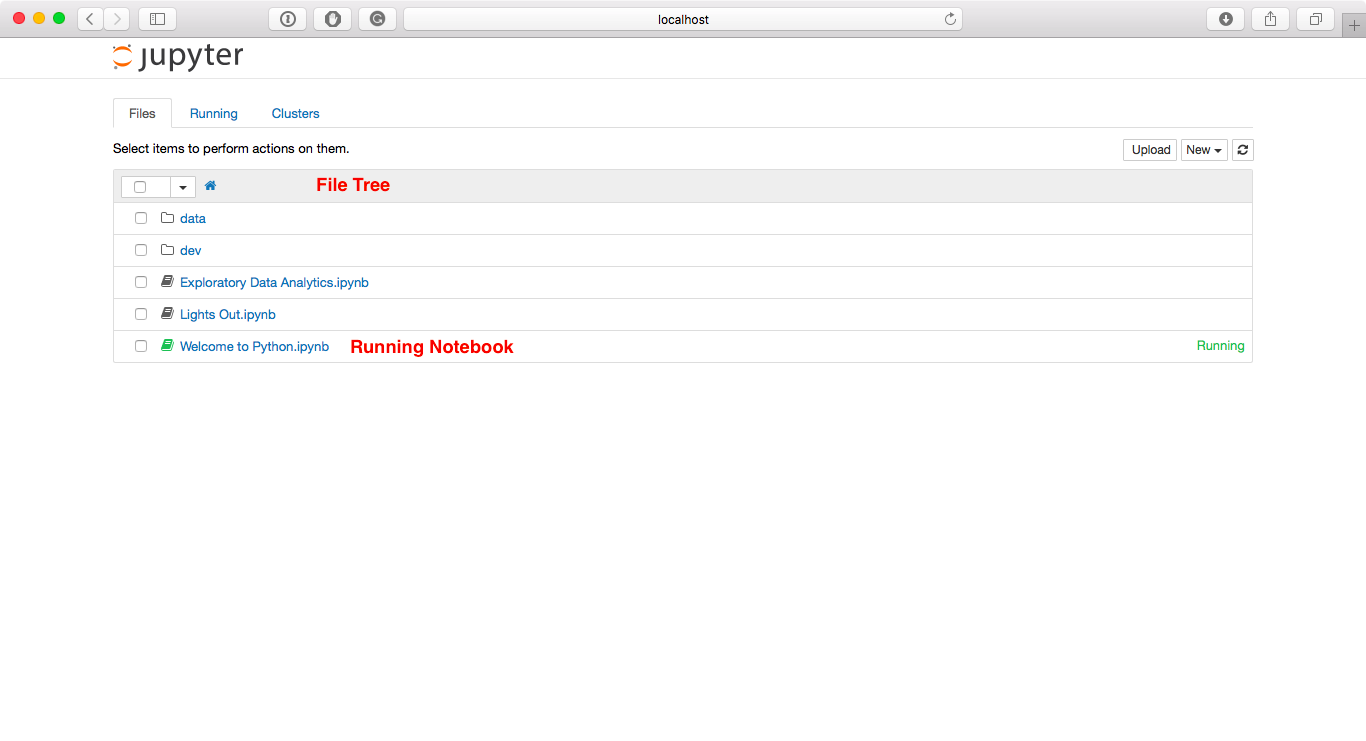
\includegraphics[width=12cm]{07_notebook/images/jupyter_dashboard.png}
\end{center}

\end{frame}

%-------------------------------------------
\begin{frame}{Jupyter}
Notebook editor

\begin{center}
    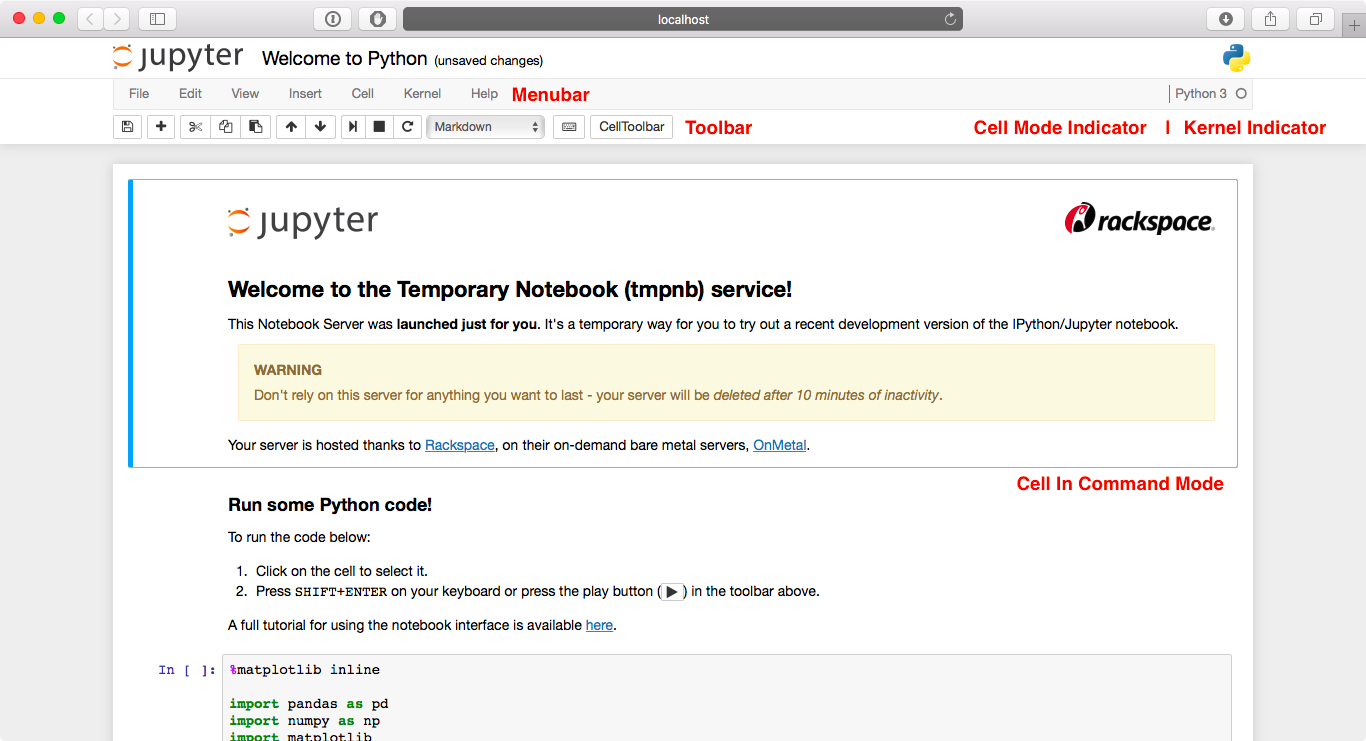
\includegraphics[width=12cm]{07_notebook/images/jupyter-notebook-editor.png}
\end{center}

\end{frame}

%-------------------------------------------
\begin{frame}{Jupyter}
Project Jupyter

\begin{itemize}
    \item A non-profit, open-source project maintained by a \textbf{strong} Community
    \item Adopted by the biggest in the Cloud industry (Google, Microsoft, Amazon...)
    \item And financed by the biggest (Google, Microsoft, EU Horizon 2020 program, Alfred P. Sloan Foundation...)
\end{itemize}

Inside the Python community (snakemake, conda...)\newline

Integration with GitHub since 2015 (renderer)

\end{frame}

%-------------------------------------------
\begin{frame}{Jupyter}
Nbviewer : a static renderer for Jupyter notebooks

\begin{center}
    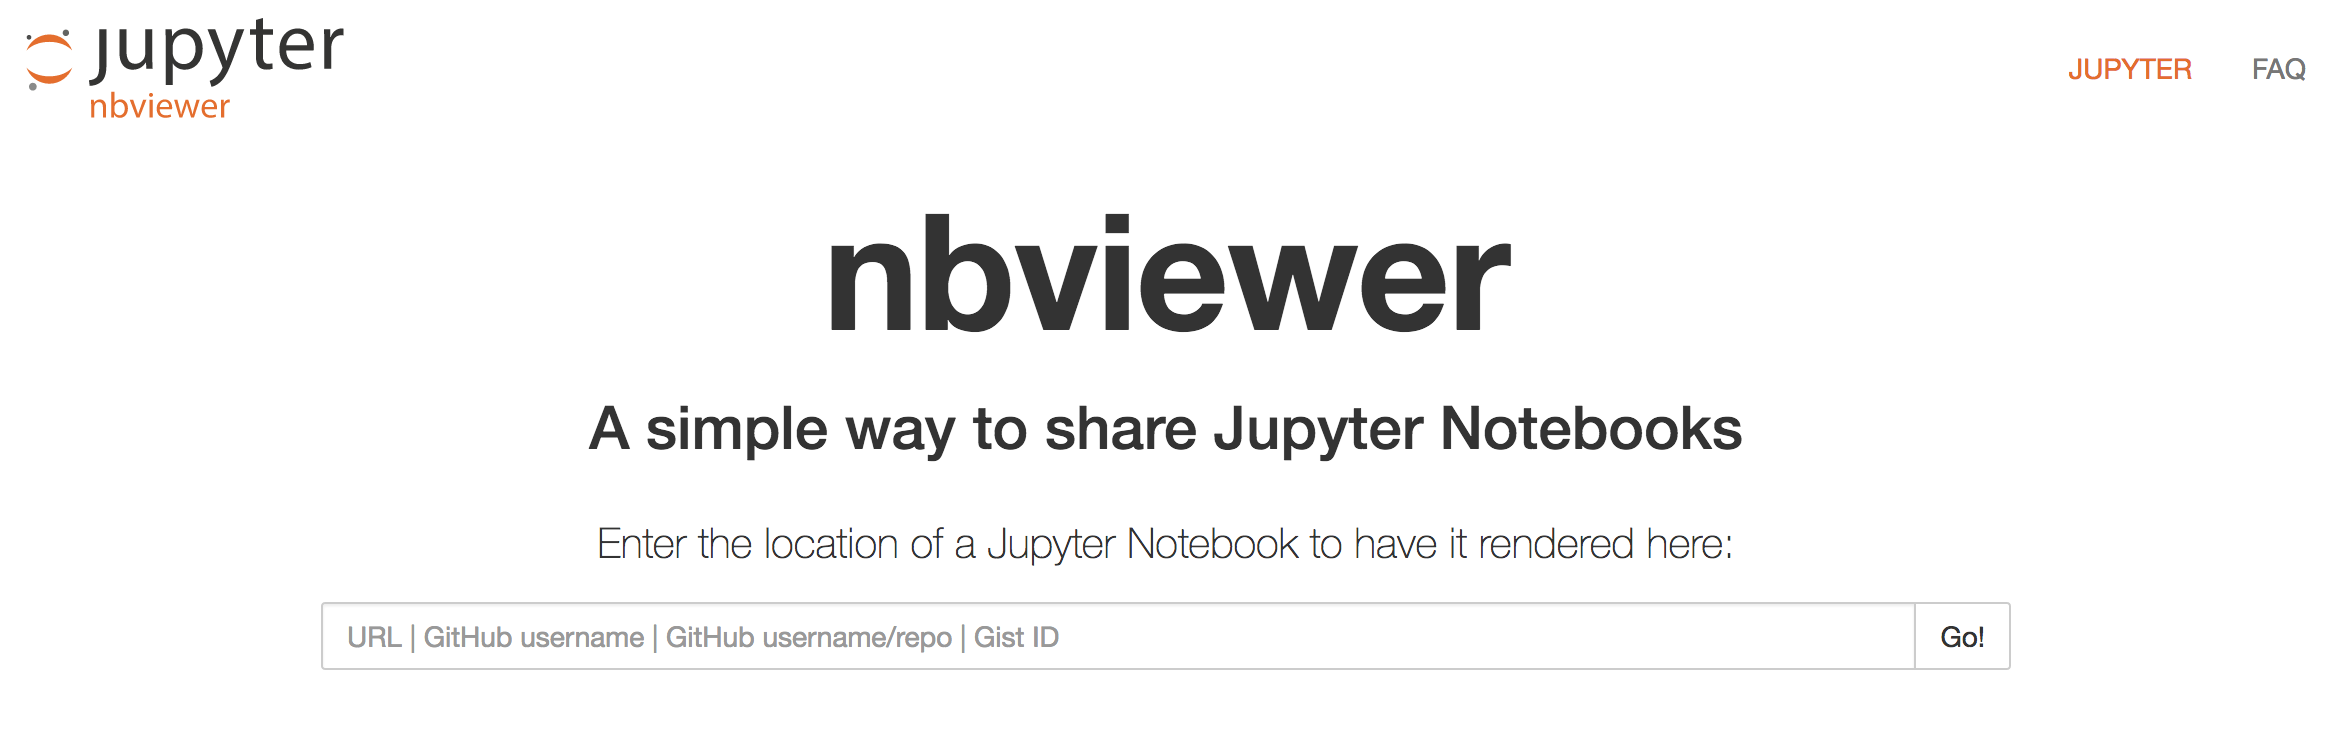
\includegraphics[width=12cm]{07_notebook/images/nbviewer.png}
\end{center}

\url{https://nbviewer.jupyter.org/}
\end{frame}

%-------------------------------------------
\begin{frame}{Jupyter}
Jupyter + Docker = binder

\begin{center}
    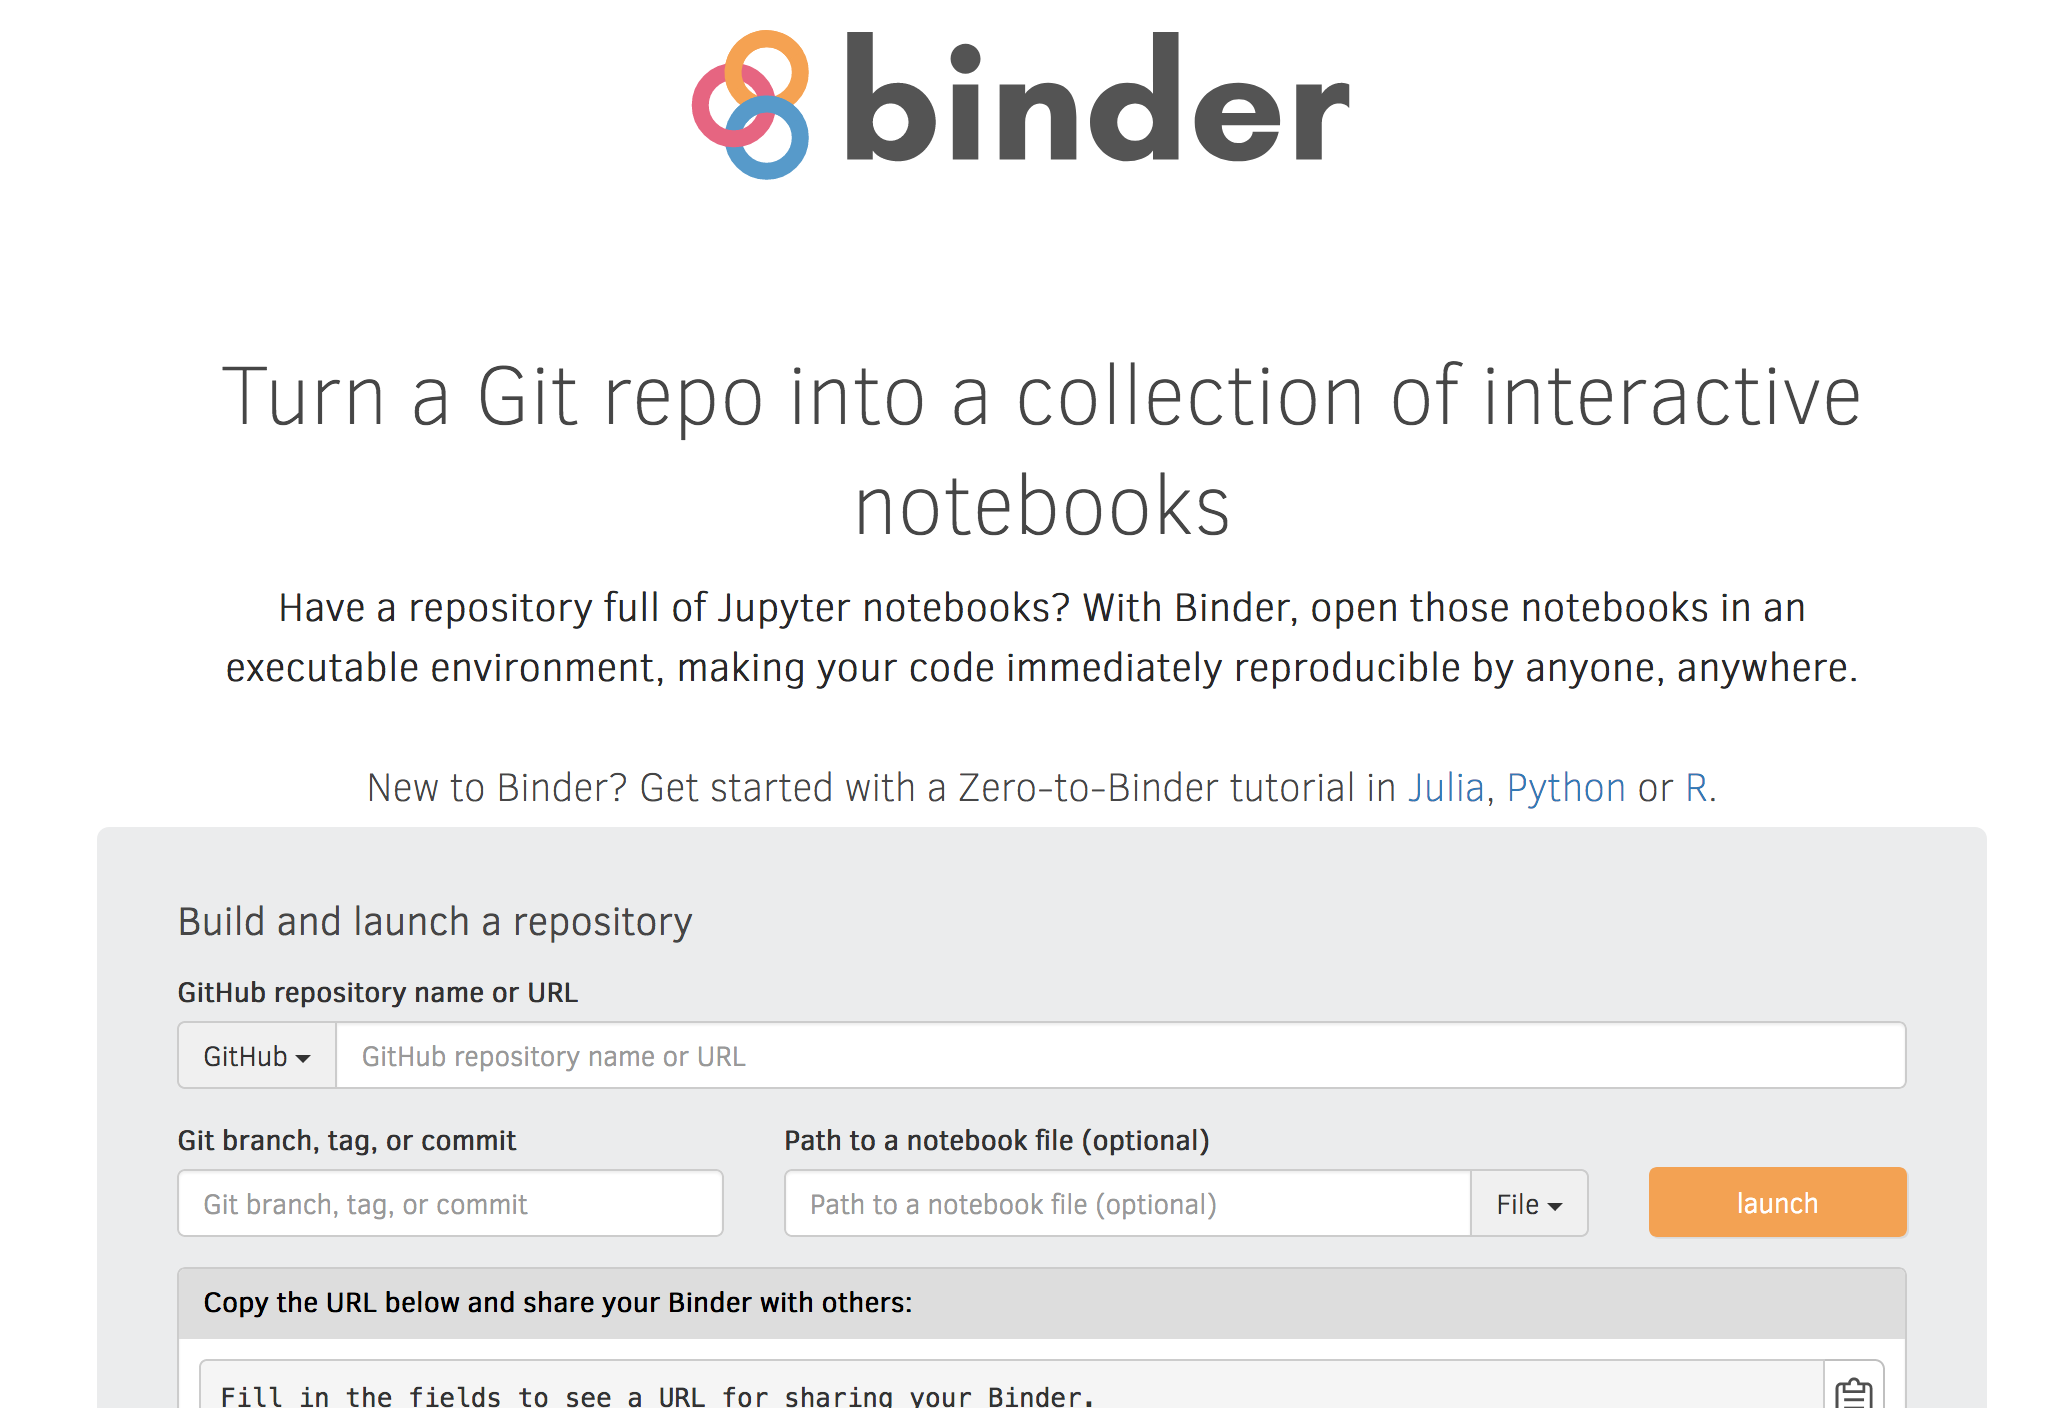
\includegraphics[width=10cm]{07_notebook/images/binder.png}
\end{center}

\url{https://mybinder.org/}
%https://mybinder.readthedocs.io/en/latest/
\end{frame}

%-------------------------------------------
\begin{frame}{Jupyter}
More to come : Jupyter Lab 1.0

\begin{center}
    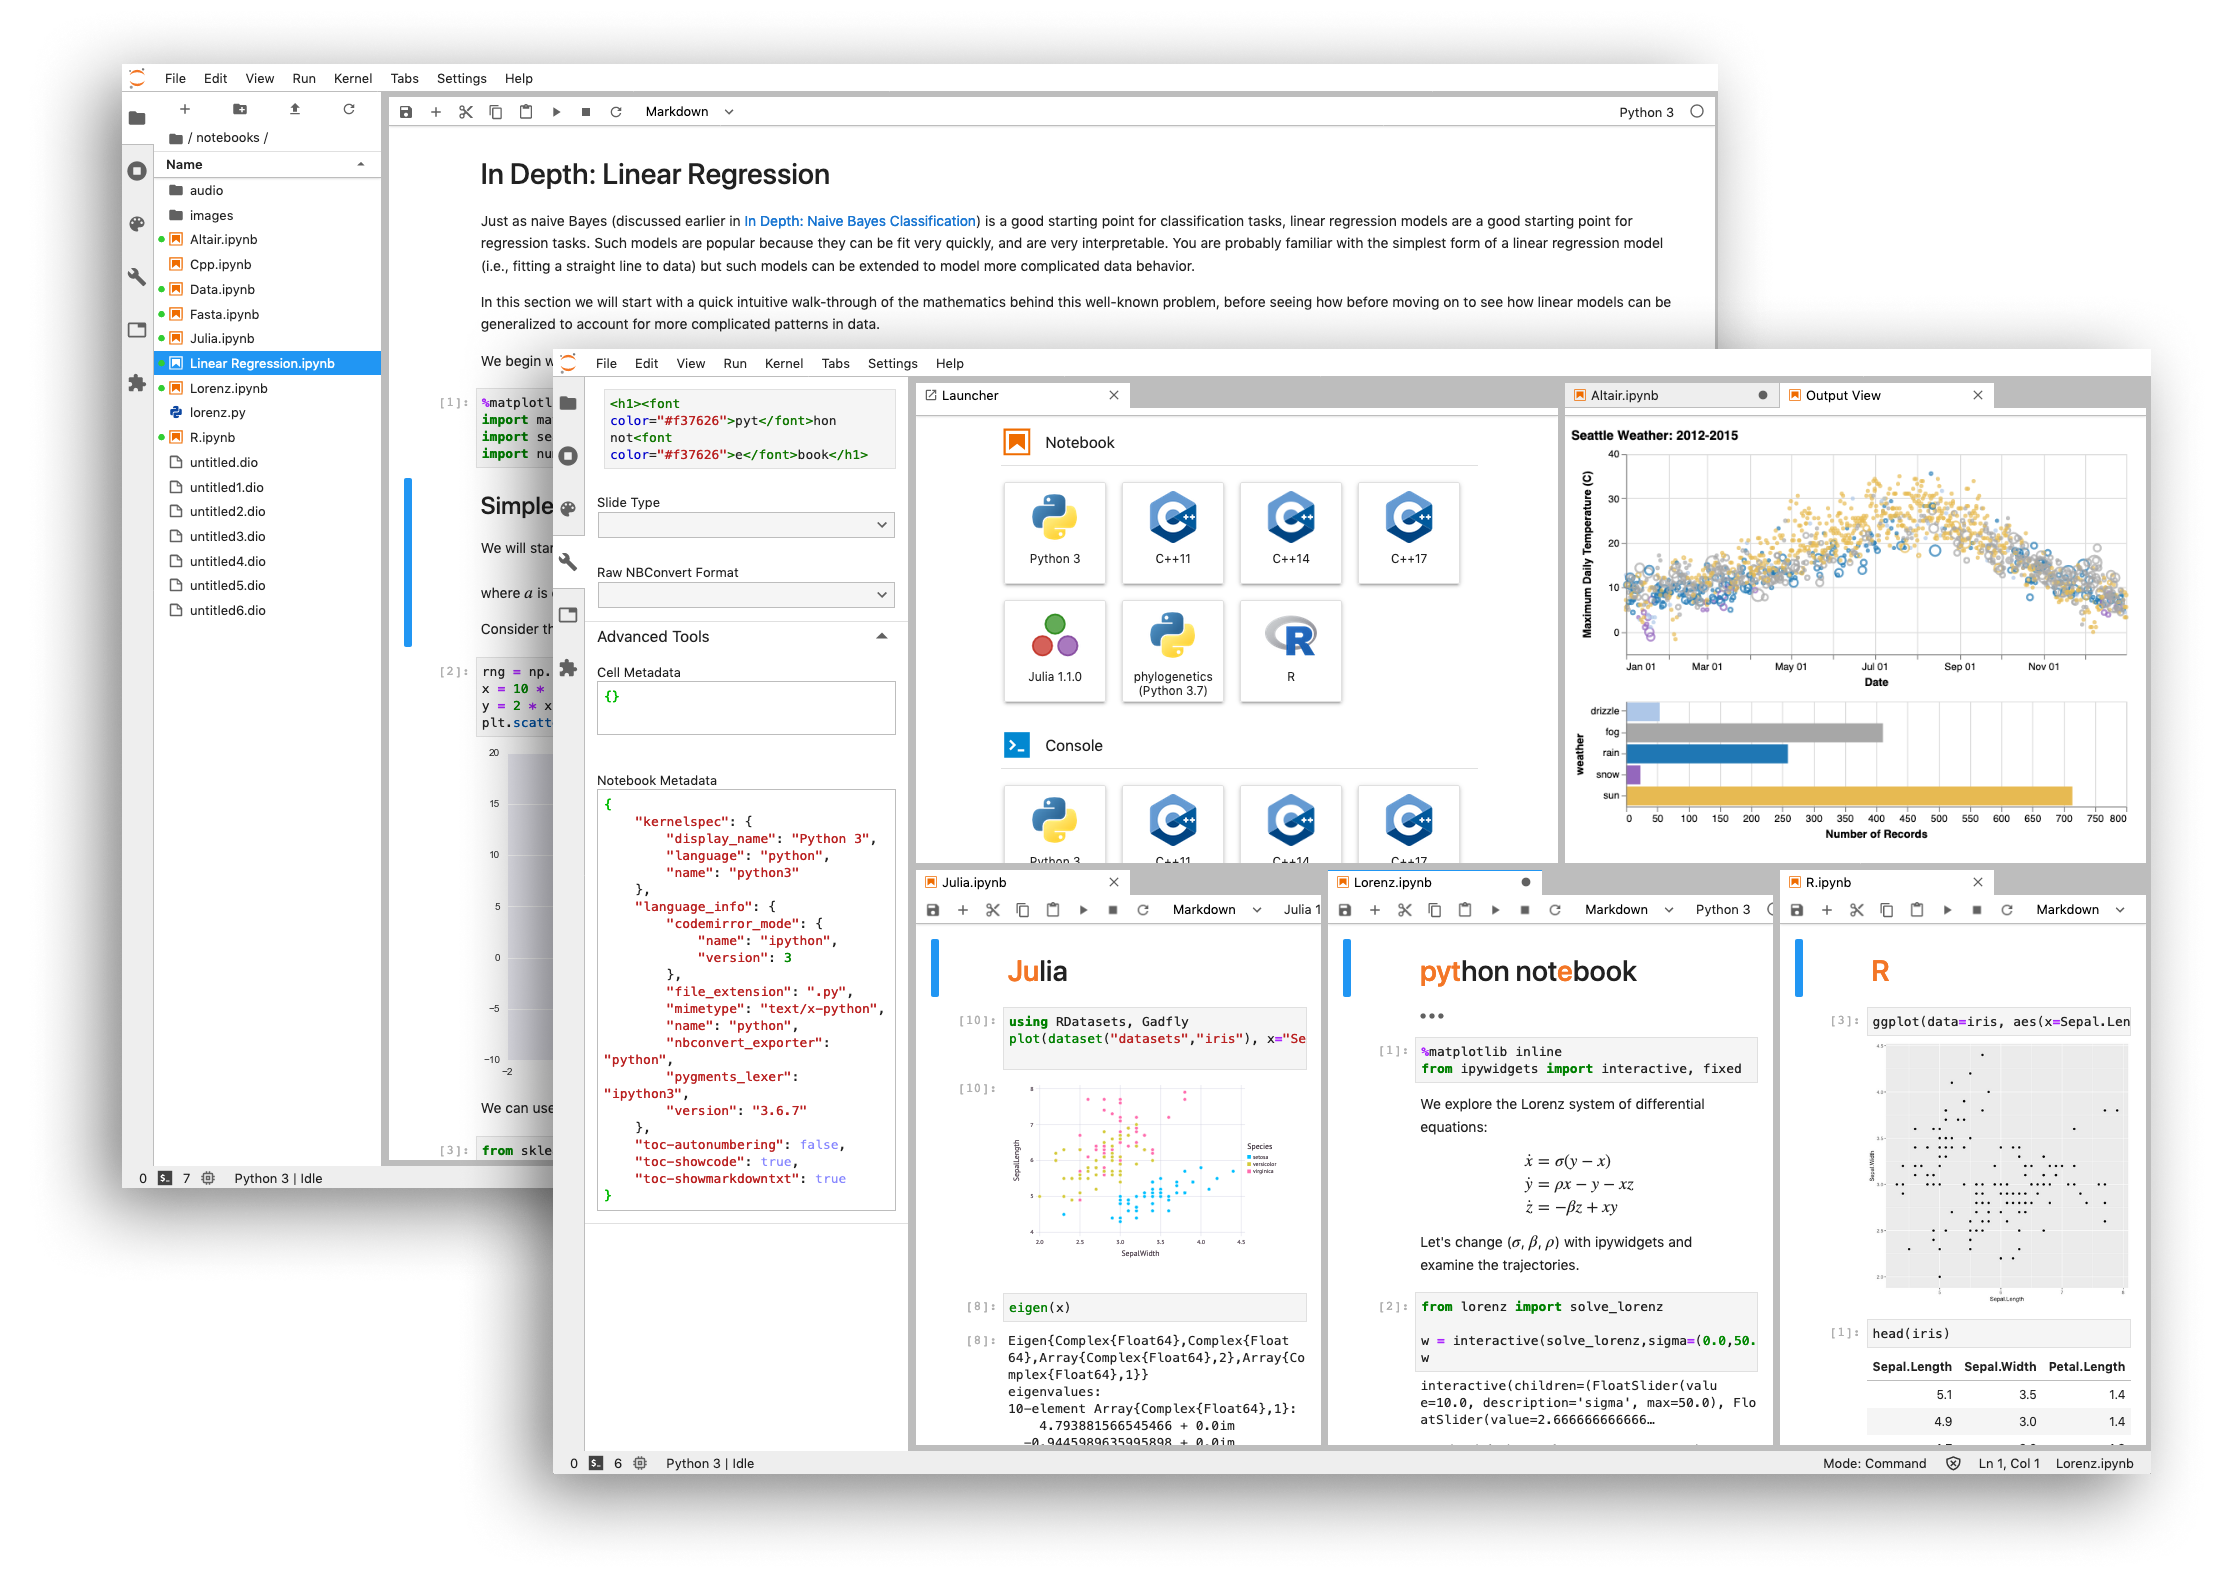
\includegraphics[width=10cm]{07_notebook/images/jupyter_labpreview.png}
\end{center}

\end{frame}

%-------------------------------------------
\begin{frame}{Conclusion ?}
Who's the best? \newline \pause 

It depends... \pause

\begin{itemize}
    \item<2-> R analyses? Go for RMarkdown/RStudio
    \item<3-> R analyses for a publication ? Consider Jupyter with an R kernel
    \item<4-> Python analyses ? Why do you even ask... 
\end{itemize}

\end{frame}

%-------------------------------------------
\begin{frame}{Practical session}
%-------------------------------------------
\begin{block}{Analysis workflow}
    \includegraphics[width=12cm]{01_introduction/images/FAIR_RNAseq_WF.png}\\
green=input, blue=tool
\end{block}
\footnotesize{
\begin{description}
    \item[fastqc] control quality of the input reads
    \item[bowtie2] reads mapping on the genome sequence
    \item[samtools] mapped reads selection $\&$ formatting
    \item[HTseq] count table of mapped reads on genes (annotations)
    \item[DESeq2] statistical analysis: genes list having differential expression
\end{description}
}
\end{frame}

%------------------------------------------------------------
\begin{frame}{Practical session}
Savoir FAIRe

\begin{itemize}
  \item Markdown
  \item Learn the structure of an Rmd file
  \item Turn a script into a notebook
  \item Extend the notebook with new functionalities
  \item Bonus: introduction to Jupyter
\end{itemize}
\end{frame}

